\section{\textbf{TORCS Environment and SCRC}} \label{sec:Environment}

	The Open Racing Car Simulator (TORCS)~\cite{TORCS} is a widely used platform for benchmarking AI, renowned for
	its	highly credible physics modeling engine and yet user-friendly interface for car racing simulation. One of
	the	many other qualities of this open-source simulator is its portability, concerning multi-platform environments
	- such as different operational systems and architectures - and support to the programming languages C and C++. A
	brief introduction to this environment and to a well-known simulated car racing competition that resorts to it is
	presented in this section.

\subsection{TORCS as platform, interface and environment} \label{subsec:TORCS}
	
	TORCS deals with a robotic simulation in the format of car racing. It serves both as an ordinary AI game and a
	research platform~\cite{2009}, providing through the interface with its competitions a complete sensor-based
	interaction system in which the developer is able to interpret received parameters of the car - such as speed in
	X, Y and even Z axes - and construe them in order to control the car through programming its actuators, some of
	which are acceleration and steering. This behaviour is widely embraced when it comes to artificial intelligence
	methods - a set of inputs to result in a set of outputs.
	
	Another credibility factor for this platform is its non-punctual cars, each of which possess a body with sensors
	and actuators, as mentioned earlier, and interact with other cars in the environment by a life-like collision
	system. Nevertheless, TORCS is still a simulator, and its limitations, along with the defined racing environment
	and the modeled robotic car, are more than likely to affect any results obtained. This is an inherited
	characteristic of any real-life problem simulation, what in academia is denominated \emph{reality gap}~\cite{RG}, and it stems from the simplifications attained concerning the car models, the technical features of the tracks,
	and so forth.

\subsection{The SCR Championship} \label{subsec:SCRC}

	The Simulated Car Racing Championship (SCRC)~\cite{SCR} is an example of a well-known competition which utilizes
	TORCS as interface. Being an event joining three competitions held at major scientific conferences, such as
	\emph{IEEE Congress on Evolutionary Computation}~\cite{CEC}, \emph{Genetic and Evolutionary Computation
	Conference}~\cite{GECCO} and \emph{IEEE Conference on Computational Intelligence and Games}~\cite{CIG}, it is
	an accepted	metric of evaluation in the fields of Evolutionary Computation and Computational Intelligence
	regarding Games.
	
	The SCRC features encapsulation with its interface towards TORCS, meaning there is an abstraction layer between
	the two and, in addition, some of the information about the racing execution remains hidden from the controllers,
	such as the geometrical format of the track and its category. SCRC and TORCS communicate through UDP packages,
	and each player receives information regarding the sensors of the car, some of which were already presented
	earlier on this section. Figure~\ref{Fig:1} illustrates the data available at the TORCS and client(controller) layer 
	of abstraction. \toDo{ tambem temos algumas informacoes que estao do lado do torcs, exemplo: temos acesso ao fuel }

   	\begin{figure}[h]
	\centering
	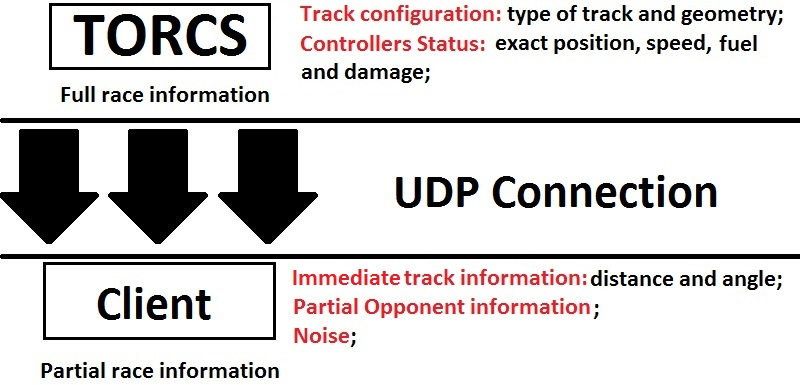
\includegraphics[width=250pt]{Figure1}
	\caption{\label{Fig:1}Available data inside TORCS and at the client.}
	\end{figure}
	
	A brief description of the sensors is as follows: the driver can use a set of sensors to acquire relative
	position, speed, and car conditions such as rpm, damage and gas. Useful information about the car during a race
	can be mined from the data provided by the said sensors; for example, there are two sets among them labeled
	\emph{track} and \emph{trackpos} that inform the position of the racer according to a desired direction and
	according to the track axis, respectively, and these two sets can be combined to inform an approximate location
	of the car regarding the racing lane.
	
	The complete sensorial input information can be found at the Simulated Car Racing Championship Competition
	Software Manual~\cite{SCRC}, within section 7.7. Noise can be incorporated to the aforementioned sensors,
	option that is inexorably present during the actual competition and will be dealt with in the section Future
	Works.

	Race tracks differ from each other concerning sensorial input if they are part of different group types, which
	are categorized into \emph{Road}, \emph{Dirt} and \emph{Oval}. The races from the SCRC take place in track types
	decided by the organization of the championship, information which is not provided to the participants and that
	may incorporate unprecedented maps. The competition adopts the following structure:
	
		\begin{itemize}
			
			\item \emph{Warm-up} - when each driver is able to explore the track and deduce information from it	at
			will, for a limited time on their own. This encourages the application of online learning techniques
			that can be useful in a race on the same track;
			
			\item \emph{Qualifiers} - a stage placing each driver in a race alone against the clock to select the best
			ones to compete in the \emph{Actual Race};
			
			\item \emph{Actual Race} - when finally the eight best drivers from the \emph{Qualifiers} race against
			each other.
			
		\end{itemize}
	
	The reason why TORCS presents itself as a satisfactory AI benchmark, in combination with SCRC, is because even
	though there is an infinity of possibilities on how the sensorial input received from the server can be
	translated into the behaviour of the actuators, they can all be compared in a race, which has a robust and steady
	scoring and evaluational system. In other words, there are many different approaches concerning how to teach the
	racer encoded by the developers to drive in a racing competition only with the information given by the sensors,
	and the metric to that issue is the performance on the race itself.

\subsection{Related Works and State of the Art} \label{subsec:Related}
	
	Some examples of awarded controllers and their driving methods will be presented in this subsection. They are
	what can be called the State of the Art among TORCS, and it is very common among them the incorporation of
	machine learning methods, along with other evolving techniques using artificial intelligence. Instinctively, as
	the nature of the problem comprises evolution by experience, learning procedures tend to enhance performance and
	competitiveness. Essentially, there are two ways of evolving controllers: Online Learning and Offline Learning,
	the first meaning that improvements are achieved during the actual race execution time and the latter that it is
	done before the competition, on the account of the developers themselves and with their own resources.
	
	The current champion of the SCR Championship is the controller \emph{Mr. Racer}~\cite{MrRacer}, and it has
	proven to be the State of the Art by winning at least the last three competitions that happened. The authors
	of this implementation adjust parameters offline through Covariance Matrix Adaptation Evolution Strategy
	(CMA-ES), use regression and low-pass filtering to reduce noise impact, distinguish normal asphalted roads
	from dirt-based ones for behavioral separation and implement an authentic opponent-handling method. Their
	Online Learning consists on a track model selection, which categorizes each track raced into dirt or road and
	chooses from databased sets of parameters the one that best fits the track and the tuning of a target speed for
	all its	corners.
	
	Another renowned controller is \emph{AUTOPIA}~\cite{AUTOPIA}. According to the founders of the
	competition~\cite{SCRC} and the authors of \emph{Mr. Racer} themselves, it is a competitive match, with the
	potential to even be the best one available, but since no entries were received from them in a while, their
	means of winning a competition were somewhat restrained. Nevertheless, assessing its performance is
	worthwhile, and its description is the implementation of a modular Fuzzy Architecture, whose division contains
	gear, steering and speed control. Their controller is optimized by means of a genetic algorithm for Offline
	Learning, and by means of landmarking the lane exit points for further speed reduction for Online Learning.
	
	These and other controller exemplifications served as criteria for the analysis and development of the
	approach presented in this paper. Aspects incorporated and adapted from them feature modularity, offline learning
	through genetic algorithms, online learning through landmarking and choosing sets of parameters for different
	categories of tracks, etc. Aspiring to design a controller capable of incorporating these features, the design of
	a model was proposed and is presented in the succeeding section.
	